% \pdfoutput=1 % (Tectonic build)
\documentclass[11pt]{article}
\usepackage[review]{acl}
\usepackage{times}
\usepackage{latexsym}
\usepackage[T1]{fontenc}
\usepackage{microtype}
\hyphenation{answer answers}
\usepackage{amsmath}
\usepackage{graphicx}
\usepackage{tikz}
\usetikzlibrary{positioning,arrows.meta}

\newcommand{\guardaudit}{\textsc{GuardAudit}}
\newcommand{\twelveB}{12B$_0$}

\title{BankShield: Fairness-Aware Safety Guardrails \\ for Indian-Language Banking AI}

\author{Anonymous ACL submission}

\begin{document}
\maketitle

\begin{abstract}
Conversational AI now serves millions of vernacular banking users in India, yet its safety layer is borrowed from English settings. We ask whether the guard is itself demographically fair, and audit six guards on Indian-context banking counterfactuals. The banking-specific evaluation exposes failures that general benchmarks miss: no guard separates coded proxy-discrimination from legitimate risk (best paired accuracy 37.5\%); several fail entirely on distressed-customer handling; and guard competence is domain-specific. We also find invariance and detection are separable: general-purpose guards stay invariant only by detecting almost none of the biased content they should catch (6--24\%), while a recent Indic guard detects it but is itself identity-biased (19\% flip). We consolidate these checks into \guardaudit{}, a reusable audit protocol, and release it with two banking benchmarks. Using BankShield as a case study, we find that it and the general guards flag none of the benign counterfactual sets (0\% flip), and its 66.7\% biased-content catch does not significantly exceed the Indic guard's 56.9\% ($p{=}0.09$); much of its competence comes from its open backbone.
\end{abstract}

\section{Introduction}
\label{sec:intro}

Conversational AI has become core financial infrastructure in India. Retail banks serve tens of millions through messaging-platform assistants in regional languages, increasingly mediated by LLMs that not merely answer but act: initiating transfers, updating KYC records, triggering account actions. The safety layer sits between a customer and their money, so an error is not a rude sentence but a financial event. A wrongly blocked request denies a customer their own account; a wrongly allowed one advances a fraud. Those most exposed are the first-time and vernacular users financial inclusion is meant to reach.

The guardrails governing these systems were built for English, and their assumptions break in Indian banking on three fronts (\S\ref{sec:problem}). Customers write in code-mixed, romanized text, and adversarial inputs exploit exactly these surface forms that English-first filters cannot read \citep{aswal2025haetbhasha}. The banking harm surface (OTP/UPI fraud, impersonation, KYC bypass, laundering) does not resemble general toxicity, while ordinary banking terms (\emph{foreclosure}, \emph{lien}) are misread as unsafe. And regulation (the Reserve Bank of India's data-localization directive, its outsourcing norms, and the DPDP Act) makes sending customer data to externally hosted models a compliance risk, so banks in our target segment require an on-premise guardrail. Beyond detecting harm, such a system must also treat customers equitably across demographic identities, a requirement existing banking safety evaluations rarely examine, and the central concern of this paper.

This reframes the problem: there is no escape hatch. Escalating a misclassified query to a larger hosted model would conflict with these institutions' on-premise data requirements, so multilingual safety shifts from \emph{coverage} (more languages) to \emph{sufficiency} (whether a compliant self-hosted system is good enough alone), and must be evaluated as the deployed system it is forced to be.

Recent work addresses Indic safety, establishing that a dedicated Indic guard outperforms multilingual baselines; in financial NLP, domain-specialized models trained on regulation-grounded data outperform general baselines on compliance tasks \citep{jiang2025intellichain,wang2025regulations}. But this work targets regulatory \emph{knowledge} and broad social harm, is trained largely on machine-translated data (stripping the code-mixing real banking attacks use), and is evaluated on held-out sets rather than in deployment. The missing question is whether the guard itself behaves fairly: whether its verdict changes when only a demographic attribute (caste, religion, region, gender) varies. Since fine-tuning can induce bias and a biased guard silently over-polices some groups, this is not optional for a regulated deployment.

We address this with BankShield, our safety framework for Indian-language banking AI, evaluated as a compliance-aware system in a live, self-hosted pilot (283 moderation events; Appendix~\ref{app:training}): a pilot, not a production deployment. Our central finding reframes what fairness means for a guard: fairness is not invariance; it is invariance without blindness, since a guard blind to a discriminatory denial is not fair to the customer denied. We argue fairness auditing should be standard in evaluating multilingual high-stakes safety guards. Our contributions:

\begin{itemize}
\item \textbf{A fairness audit of safety guards themselves.} Using \guardaudit{} (our protocol; next contribution), we audit six systems on Indian-context counterfactuals and show general-purpose guards achieve demographic invariance only by not detecting biased content, while a recent Indic guard detects it but is itself identity-biased; BankShield, by contrast, leaves benign identity content unflagged (0\% flip) while still catching biased content, a separate-axis result that rules out flag-nothing behaviour without proving joint per-example fairness (\S\ref{sec:fairness}). To our knowledge this is the first counterfactual demographic-fairness audit of Indic safety guards; prior guard-fairness audits target commercial English moderation APIs \citep{watchdogs2025}.
\item \textbf{A reusable evaluation protocol, and a system that validates it.} We consolidate the standard checks---decontamination, paired detection/over-block with CIs, and a fairness audit---into \guardaudit{} (Appendix~\ref{app:protocol}) and apply it to BankShield, a self-hosted guard with direction-aware moderation whose competence comes largely from an open backbone and whose adaptation adds biased-content detection (\S\ref{sec:direction}). We release the protocol and artifacts.\footnote{The supplementary material provides the evaluation code, prompts, decontaminated benchmark sets with item IDs, per-item prediction logs, expected metric values, environment and model-version information, and---for the fairness evaluation---the output-side discrimination probe with its 0.7 decision threshold, the disclosable policy configuration, and the scoring scripts, together with a SHA-256 manifest (a public repository will accompany the camera-ready). We internally re-executed the deployed system end-to-end; the released artifacts reproduce the reported evaluation from these frozen per-item predictions. Proprietary LoRA weights and production policy rules are not included because of commercial and security constraints, so reviewers cannot re-run model inference end-to-end; the base model (\texttt{google/gemma-4-12B-it}) is public.}
\item \textbf{Two banking benchmarks and three findings on the limits of current guards.} Grounding fairness in banking decisions (RBI Charter grounds; coded-discrimination patterns from Indian case law) and adding a direction-aware output-safety benchmark, we find (i) no guard reliably separates coded proxy-discrimination from legitimate adverse decisions; (ii) proxy-detection and group-fairness trade off (on a single benchmark, few systems); and (iii) safety competence is domain-specific. BankShield catches biased content comparably to the Indic guard but not significantly better ($p{=}0.09$), with 0\% flip on benign counterfactuals, alongside mid-pack paired calibration, reported as-is (\S\ref{sec:banking}--\S\ref{sec:policyflex}).
\end{itemize}

Where prior work asks whether an Indic guard can be built, we ask whether one is fair enough to deploy, and answer with a working system and a reusable way to measure it. On the hardest case, coded discriminatory denial, no guard including ours separates proxy from legitimate risk; there our contribution is the measurement, not a solution.

\section{The Indian Banking Safety Problem}
\label{sec:problem}

We characterize what makes safety for Indian-language banking assistants a distinct problem, and why a general-purpose guard, even one adapted to Indic languages, cannot simply be dropped into this setting.

\subsection{A domain-specific harm surface, in both directions}
\label{sec:harm}

The harms that matter in banking differ from general taxonomies. A banking assistant faces attacks whose surface form is often polite: prompt injection, fraud and social engineering (soliciting an OTP or UPI PIN, impersonating a bank officer), KYC bypass, money-laundering, none carrying toxicity markers yet exactly what a banking guard must catch. The dual failure is over-blocking: \emph{foreclosure}, \emph{lien}, \emph{encumbrance} read as threatening, and code-mixing compounds this. Generic filters thus both miss real attacks and deny service on ordinary terms; no single threshold fixes this. It needs a model whose notion of harm is domain-aligned, attending to intent and directionality, not surface offensiveness.

\subsection{Regulation, and why blocking is not the only action}
\label{sec:reg}

The RBI's storage/localization framework and outsourcing norms, together with the DPDP Act, constrain how customer data may be handled; RBI permits overseas processing subject to storage/return-to-India and deletion conditions rather than barring it outright, but the banks in our target segment adopt on-premise processing as an operational requirement. A guard sending customer messages to a cloud-hosted model thus raises outsourcing and auditability concerns for these institutions; they require on-premise deployment, which forces a self-hosted guard sufficient on its own. The RBI framework further expects fairness testing and explainability. Safety here is also not binary: a customer in distress or with a grievance is not producing content to block, and refusing it is itself a harm. BankShield therefore distinguishes \emph{allow}, \emph{block}, and \emph{route to human}, which matters for measurement, since counting routed grievances as over-blocks would misrepresent the system (\S\ref{sec:results}).

\section{Related Work}
\label{sec:related}

We situate our work (safety for AI deployed in Indian-language banking) against three adjacent lines, each a foundation we build on rather than the space our contribution occupies.

\paragraph{Guard models and safety evaluation.} The prevailing approach to LLM safety is an external moderation layer returning a verdict on a prompt or response, e.g.\ Llama Guard \citep{inan2023} and ShieldGemma \citep{zeng2024shieldgemma}, fine-tuned on datasets such as AEGIS \citep{ghosh2024aegis} and BeaverTails \citep{ji2023}. This literature also produced instruments we adopt, notably XSTest \citep{rottger2024xstest}, which isolates exaggerated safety, the over-refusal of benign but sensitive prompts. This work is overwhelmingly English, with taxonomies that do not transfer across languages \citep{adilazuarda2024}, and reports safety as an aggregate score, whereas a guard's behaviour is visible only in the pair: harm caught and legitimate content wrongly blocked (\S\ref{sec:setup}).

\paragraph{Multilingual and culturally-aware moderation.} A recent shift extends safety beyond English: for the Indic space, CultureGuard \citep{joshi2025cultureguard} and related work establish that Indic safety is distinct (harm is socio-culturally situated) and release Indic-specialized guards, the closest prior work to ours and a foundation we build on. Recent multilingual guards (PolyGuard \citep{kumar2025polyguard}, Qwen3Guard \citep{qwen3guard2025}, and the LoRA-adapted SEALGuard \citep{sealguard2025}) broaden language coverage but are neither domain-specialized nor fairness-audited. All of these, Indic and multilingual alike, are by design general-purpose guards evaluated as research artifacts: they do not target a specific domain, are not evaluated as deployed systems under regulatory constraint, and do not audit whether the guard's own verdicts are demographically biased: scope boundaries that describe the space our work occupies.

\paragraph{Domain-specific, deployed, and fairness-aware safety.} Three further threads bound our contribution. Most central is fairness of the guard: prior Indic-safety work treats identity as a category of harm to detect \citep{sahoo2024indibias,nawale2025fairitales,khandelwal2024indianbhed}, and counterfactual and perturbation-based fairness analyses exist for English toxicity classifiers \citep{dixon2018,prabhakaran2019,garg2019,kusner2017}, but no prior work asks whether an Indic guard is itself biased when only a protected attribute changes. The other two are deployment (research models do not face the latency, localization, and auditability of a live banking system) and domain: FinGuard \citep{dou2026finguard} targets regulatory-compliance violations, not the guard's own fairness, and covers no Indic language; banking's harm surface remains largely unexplored for Indic.

\paragraph{Positioning.} Prior work establishes that Indic safety matters and that a dedicated Indic guard is achievable, foundations we build on. Our contribution is not another Indic guard but \guardaudit{}, an evaluation framework for the fairness of deployed multilingual banking safety systems, demonstrated through BankShield (Table~\ref{tab:positioning}). Concurrent submissions by overlapping authors study the same Indian banking-assistant setting from complementary angles---code-mixed language identification and intent understanding under noise \citep{anonwnut2026a,anonwnut2026b}---but address neither the guard's safety behaviour nor its demographic fairness, and share none of the benchmarks, the guard system, or the audit protocol evaluated here; we disclose them per the anonymity policy for related concurrent work.



\section{BankShield}
\label{sec:system}

Conceptually, BankShield is a cascaded safety system mediating each turn between a customer and an assistant. A message undergoes deterministic normalization, then a multilingual classifier and lightweight probes; a configurable policy engine maps their outputs to one of three actions: allow, route to a human, or block (Figure~\ref{fig:pipeline}, Appendix~\ref{app:arch}). As a guard on regulated data we release evaluation artifacts but not production rule sets or weights, for which a commercial/security exception request is pending with the workshop organizers. We emphasize the decisions distinguishing BankShield from a general-purpose guard sharing its backbone; fairness in particular emerges from direction-aware moderation (\S\ref{sec:direction}) and per-category policy (\S\ref{sec:threeway}) together.



\subsection{A cascaded, cost-aware pipeline}
\label{sec:cascade}

Each message passes through a short cascade. A \emph{deterministic lexical filter} normalizes the text (inserted spacing, leetspeak, repetition) and blocks on exact lexicon match at zero false-positive cost. The classifier (\S\ref{sec:backbone}) then emits a category and calibrated severity in one pass, lightweight probes (\S\ref{sec:probes}) score dimensions warranting independent re-trainable detectors, and a policy engine (\S\ref{sec:threeway}) maps these to one of three actions, keeping the decision auditable; unambiguous lexical matches (rare in practice, so most traffic reaches the classifier) block at zero model cost.

\subsection{Backbone and adaptation}
\label{sec:backbone}

We use an open, mid-sized backbone because it can be served on-premise while retaining multilingual capability (a requirement, not a preference) under \S\ref{sec:reg}. The classifier is a LoRA-adapted \texttt{gemma-4-12B-it}\footnote{Gemma~4 (\texttt{google/gemma-4-12B-it}, \url{https://huggingface.co/google/gemma-4-12B-it}) is a public Google release; a distinct, later model than the \texttt{gemma-3-4b-it} the Indic guard uses, not a typo.} in 4-bit (NF4) quantization, producing category and severity by a single deterministic pass (log-probabilities over fixed label tokens, not free-form generation); hyperparameters are in Appendix~\ref{app:training}. The general-purpose Indic guard we compare against uses a smaller, earlier \texttt{gemma-3-4b-it} backbone; to isolate the effect of adaptation rather than scale, our base-model reference in \S\ref{sec:results} is the same \texttt{gemma-3-4b-it} backbone the competitor builds on, un-adapted.

\subsection{Direction-aware moderation}
\label{sec:direction}

BankShield moderates inputs and outputs differently. The central asymmetry concerns discrimination: it detects it on the \emph{output} side (assistant responses) but does not flag a customer's \emph{input} as discrimination, because the customer is the protected party, not the source of harm: flagging their identity mention or grievance as a violation would punish the users the system serves. This choice about \emph{whose} safety the guard protects underlies the fairness behaviour of \S\ref{sec:fairness}.

\subsection{Lightweight probes}
\label{sec:probes}

Three probes, each a logistic model over multilingual E5 sentence embeddings \citep{wang2024e5} from an on-premise encoder (preserving the localization constraint of \S\ref{sec:reg}), retrainable in seconds and independent of the 12B model, score dimensions warranting dedicated, quickly-adjustable detectors: \emph{grievance}, \emph{discrimination} (output side), and \emph{abuse-elicitation}; a fourth signal, the deterministic \emph{lexical filter} (\S\ref{sec:cascade}), is rule-based. Separating these from the main model lets an operator adjust a behaviour (say, grievance-routing sensitivity) without retraining the classifier or other probes.

\subsection{A three-way action model}
\label{sec:threeway}

BankShield does not treat safety as binary: its policy engine maps each message to \emph{block}, \emph{route-to-human}, or \emph{allow} by per-category thresholds and probe outputs. Distress and grievance signals (self-harm, complaints, consent-sensitive requests, abuse-elicitation) trigger \emph{routing}, not a block: a customer in distress must be escalated, not refused. This also matters for measurement (\S\ref{sec:results}): we count only \emph{block} as a refusal, treating routing as designed escalation.

\subsection{Per-tenant policy without retraining}
\label{sec:tenant}

The model and probes are shared, but policy is per-institution: category strengths, actions, moderation directions, probe thresholds, and denied topics are set per-tenant and tuned to a bank's risk appetite without retraining, letting one deployed system serve institutions with differing compliance requirements.

\subsection{Training-data stance}
\label{sec:data}

Driven by the privacy and localization constraints of \S\ref{sec:reg}, BankShield is trained without machine translation and without real customer data. Its $\approx$172K-example corpus (51\% safe, 49\% unsafe) is 99.6\% synthetic, with the remaining 0.4\% (686 items) drawn from public benchmarks; all are authored directly in-language rather than translated. By script, 67\% is Latin (English and romanized code-mix) and 33\% native Indic (Tamil, Kannada, Telugu $\approx$ 9\% each; Devanagari 5\%; Bengali $<$ 1\%). Authoring in-language preserves the code-mixing and romanization real banking attacks use and a translation pipeline does not reproduce (Appendix~\ref{app:crosslang}); the public supplement is the source of the Hindi contamination we detect and exclude (Appendix~\ref{app:decon}).

Four design decisions distinguish BankShield from a general-purpose guard: (i) a cascaded architecture for on-premise deployment, (ii) direction-aware moderation that protects rather than polices the customer, (iii) lightweight retrainable probes, and (iv) a three-way policy separating blocking from human escalation. The biased-content detection of \S\ref{sec:fairness} follows from (ii) together with the adapted classifier and the trained discrimination probe (ablation in Appendix~\ref{app:training}).

\section{Experimental Setup}
\label{sec:setup}

Our evaluation is designed so that every reported figure is supported by released per-item logs or, where competitor logs were not retained, by frozen aggregate counts, and is robust to the decontamination and paired-metric requirements of \S\ref{sec:discussion}; public baselines can be rerun, while BankShield's own inference cannot be regenerated end-to-end without the proprietary LoRA weights and production policy rules.

\subsection{Decontamination and neutrality}
\label{sec:decon}

A guard evaluated on data resembling its training set can report misleadingly favourable numbers. Every evaluation set below is decontaminated against BankShield's training data: we remove any item that exactly matches a training example, and any whose word-level (whitespace-tokenized) Jaccard similarity to the nearest is $\geq$ 0.70 \citep{lee2022}, catching paraphrase leakage rather than only verbatim overlap (counts in Appendix~\ref{app:decon}).

\subsection{Paired-metric protocol}
\label{sec:paired}

For each system we report the over-block rate (benign items wrongly flagged unsafe) and recall (unsafe items correctly flagged) on paired benign and unsafe sets, never a detection figure alone, with Wilson 95\% confidence intervals throughout since several subsets are small. Because the key comparisons are between systems scored on the same items, we assess significance with McNemar's exact (binomial) test on paired per-item predictions; for the small number of unpaired aggregate comparisons we use Fisher's exact test. We believe reporting detection and over-block together, with paired significance, should become standard practice for financial safety systems. For BankShield's three-way decision (\S\ref{sec:reg}) we apply one convention throughout: for \emph{harmful-content catch}, a block or a safe-directed route counts as a positive (a route escalates the harm to a human rather than ignoring it); for \emph{benign over-block}, only a block counts (routing is a designed escalation, not a refusal); routing is additionally reported separately, and block-only figures are given alongside where they differ (e.g.\ output-safety catch $95.5\%$ block-or-route vs $93.9\%$ block-only).

\subsection{Datasets}
\label{sec:datasets}

We evaluate on both external and domain-specific data.

\paragraph{External calibration data.} We use XSTest \citep{rottger2024xstest}, 250 benign-but-sensitive prompts paired with 200 genuinely unsafe contrasts, as a standard, language-neutral probe of exaggerated safety, independent of any system's training data.

\paragraph{Benign banking data.} To measure over-blocking on legitimate requests, we use 200 benign English banking queries from Banking-77 \citep{casanueva2020}, a public intent-classification corpus with no India-specific training lineage, and 74 author-constructed benign Hindi/Hinglish banking queries, written by bilingual annotators and decontaminated as in \S\ref{sec:decon}. These isolate the failure mode of \S\ref{sec:harm}: refusing ordinary banking language.

\paragraph{Native-script data.} We include 40 benign native-script (Devanagari and Tamil) items to test whether calibration depends on script rather than content.

\paragraph{Fairness data.} For the counterfactual audit (\S\ref{sec:fairness}), we sample 1,056 items from BharatBBQ \citep{tomar2025bharatbbq}, an Indian-context bias benchmark: from this pool we draw 185 benign identity-mention and 123 biased items, and construct 160 minimal-pair counterfactual sets over religion, caste, region, and gender in which only the protected attribute varies while content is held constant. The same matched content, in stereotype-consistent and stereotype-violating framings, supports the direction-asymmetry analysis of \S\ref{sec:fairness}.

\paragraph{Attack data.} To measure recall on genuine banking attacks, we use 89 adversarial banking prompts spanning injection, fraud/OTP solicitation, KYC bypass, money-laundering, account-takeover, and officer impersonation, in English (35), Hindi (27), and romanized Hindi (27), authored by bilingual annotators to reflect deployment attack typologies (no real customer messages or logs are used) and decontaminated per \S\ref{sec:decon}.

Full per-dataset and per-language item counts are given in Appendix~\ref{app:stats}.

\subsection{Systems compared}
\label{sec:systems}

We compare six systems on identical decontaminated data: BankShield (12B, proposed); L3Cube-IndicGuard \citep{bramhecha2026} (4B, Indic-specific); Llama Guard 3 \citep{grattafiori2024} (8B) and WildGuard \citep{han2024wildguard} (7B), two general-purpose guards; and two un-adapted backbones (the \texttt{gemma-3-4b-it} base the Indic guard builds on, and the \texttt{gemma-4-12B-it} backbone BankShield adapts) so adaptation can be isolated from scale (\S\ref{sec:fairness}). Each competitor runs with its own released inference code; Prompt-Guard (86M) was excluded as scope-mismatched (Appendix~\ref{app:baselines}). Consistent with the workshop's open-research policy, we release our evaluation code, prompts, decontaminated benchmark sets, and fairness minimal-pair templates, and withhold the production rule sets and model weights of a deployed financial guard. All systems use greedy decoding, parsed into the block / route / allow decision space per Appendix~\ref{app:parsing}. The banking-fairness and output-safety evaluations (\S\ref{sec:banking}--\S\ref{sec:outputsafety}) extend this panel with three further deployed guards, AWS Bedrock Guardrails, NVIDIA NemoGuard, and Prompt-Guard-2 (86M, included here as a lightweight floor rather than a scope-matched guard), and use the current \emph{Llama Guard 4} (12B) in place of the Llama Guard 3 (8B) of the attack-recall and BharatBBQ panels (Tables~\ref{tab:main} and~\ref{tab:fairness}); we note the Llama version differs across the two evaluation panels.\footnote{Llama Guard by panel: version~3 (8B) in Tables~\ref{tab:main} and~\ref{tab:fairness}; version~4 (12B) in Tables~\ref{tab:banking} and~\ref{tab:outputsafety}, reflecting the current release when each panel was built.}

\section{Results}
\label{sec:results}

Our results test three claims: (H1) BankShield is a competent guard, competitive with the strongest systems, traced largely to its open backbone (\S\ref{sec:competence}); (H2) it combines low counterfactual flip with biased-content detection, reported as two separate axes rather than a joint guarantee (\S\ref{sec:fairness}); (H3) detection holds beyond English (Appendix~\ref{app:crosslang}).

\subsection{Language and domain competence}
BankShield is a competent banking guard: it matches or exceeds the strongest available systems on in-domain attack recall and benign over-refusal, and the ablation attributes most of this competence to its open backbone, with adaptation adding targeted detection (full per-system and per-language breakdown in Appendix~\ref{app:competence}). An external seven-benchmark panel (Table~\ref{tab:extcompetence}) confirms this: BankShield attains the highest harm recall of any system compared, at the highest over-block cost. We focus the main text on the fairness findings, where the systems diverge most.
\subsection{Fairness: does the verdict depend on identity?}
\label{sec:fairness}
We first audit fairness on the general BharatBBQ benchmark, scoring each guard on flip (verdict change under identity substitution, on 160 \emph{English} minimal-pair sets), biased-content catch, and benign over-flag (the catch and over-flag sets span English and Devanagari Hindi, $\sim$54/46\%; Table~\ref{tab:fairness}). The result that organizes the paper: invariance and detection are separable, and BankShield alone attains low flip together with high catch, reported as two separate-axis measurements (flip on the counterfactual sets, catch on the biased set) rather than joint per-example fairness. Detection is uneven by language: over-flag 4.0\% (en) vs 5.9\% (hi) and catch 81.6\% (en) vs 42.6\% (hi), a competence gap we flag in Limitations. Per-attribute detail is in Appendix~\ref{app:fairness}.

\subsection{From general bias to banking decisions}
\label{sec:banking}

BharatBBQ is general; the discriminatory loan denial motivating this paper is not among its items. We construct a banking-specific fairness benchmark (256 items, in English, released); the code-mixed stress our thesis concerns is carried by the output-safety set below (35\% Hinglish) and the romanized attack set (\S\ref{sec:systems}), and extending the coded-fairness items to code-mix is future work. Protected grounds follow the RBI Charter \citep{rbicharter2014} (religion, caste, gender, age, physical ability), extended with region---not an RBI-enumerated ground but a discrimination axis in BharatBBQ and Indian case law; coded items instantiate proxy-vocabulary patterns catalogued as discriminatory in \emph{Sukanya Shantha v.\ Union of India} \citep{sukanyashantha2024} and the SC \emph{Handbook on Combating Gender Stereotypes} \citep{schandbook2023}. The benchmark has three tiers: 144 minimal-pair \emph{flips} (attribute varied, decision fixed); 32 \emph{explicit} catch items (denial attributed to identity); and 40 \emph{coded} pairs (36 denial-type and 4 \emph{selective-friction}, where the adverse action is added procedural screening rather than an outright denial). Each coded pair matches a biased message whose adverse decision rests on a group-proxy (``applicants of your background lack repayment discipline'') with a control justifying the same decision by a documented fact (``more than two missed EMIs''). Items are decontaminated (max Jaccard 0.33); Catch counts a block or discrimination flag; the control false-flag rate counts a wrongly flagged control.

\begin{table}[t]
\centering
\small
\setlength{\tabcolsep}{3pt}
\resizebox{\columnwidth}{!}{%
\begin{tabular}{lccccc}
\hline
\textbf{System} & \textbf{expl.} & \textbf{coded} & \textbf{ctrl-FF} & \textbf{paired} & \textbf{flip} \\
\hline
BankShield    & \textbf{100} & 97.2 & 75.0 & 20.0 & 5/48 \\
WildGuard     & 57.7 & 47.2 & 5.6 & \textbf{37.5} & 13/48 \\
AWS Guard.    & 65.4 & 2.8 & 0 & 2.5 & 2/48 \\
NemoGuard     & 61.5 & 0 & 0 & 0 & 0/48 \\
Llama Guard 4 & 23.1 & 5.6 & 0 & 5.0 & 6/48 \\
PromptGuard-2 & 0 & 0 & 0 & 0 & 0/48 \\
\hline
\end{tabular}}
\caption{Banking fairness benchmark, output mode, in \%. \emph{expl.}\ / \emph{coded}: catch on explicit / coded-proxy discrimination (explicit over 26 items, after excluding 6 malformed templates; \emph{coded} over the 36 denial-type items); \emph{ctrl-FF}: control false-flag rate on the 36 legitimate controls (expert-validated; Appendix~\ref{app:stats}); \emph{paired} ($n{=}40$, the 36 denial-type plus 4 selective-friction pairs): fraction where the biased half is flagged \emph{and} the control cleared; \emph{flip}: sets (of 48) whose verdict changes across group substitution (lower is fairer). Interpretation in \S\ref{sec:banking}. Wilson 95\% CIs in Appendix~\ref{app:ci-extra}.}
\label{tab:banking}
\end{table}

Table~\ref{tab:banking} yields three findings. First, on the \emph{paired} metric (the discriminating test, requiring a system to flag proxy-discrimination \emph{and} clear the matched legitimate decision), no system does well: the best, WildGuard, reaches 37.5\%. Explicit discrimination is largely caught (BankShield 100\%, others 23--65\%); coded proxy-discrimination is where the field breaks down. Second, the failures are structured, not random. AWS and the three open guards are \emph{proxy-blind}: they both-clear most pairs, never flagging the coded bias (paired 0--5\%). BankShield is the mirror image: it both-\emph{flags} most pairs (paired 20.0\%), catching the proxy language but firing equally on the legitimate control: it detects ``adverse banking message,'' not discrimination specifically. The 40 legitimate controls are expert-validated (two independent experts accepted 40/40 and 39/40; Appendix~\ref{app:stats}), so this 75.0\% is a genuine control false-flag rate. A sensitivity sweep confirms this is not a calibration artifact: no threshold separates proxy from actuarial reasoning, because false-flags decompose across detectors that share adverse-tone features (Appendix~\ref{app:sweep}). These catch figures are not an artifact of the three-way decision: counting only \emph{block} (not route) as a flag leaves explicit catch unchanged at 100\% and coded catch at 94.4\%, versus 97.2\% when routing is included.

\paragraph{A proxy-detection / group-fairness tension.} Third, the one partial separator pays for it. WildGuard reaches the best separation (37.5\%) but is the \emph{only} system with substantial identity-conditioned flipping (13/48 flip-sets; others $\leq$6), and its identity-firing is bimodal: concentrated in \emph{communal} classes (religion, caste, region), while on gender it separates with \emph{zero} identity-attention cost. The tension is real where identity is communal, but gender shows it is not an architectural necessity (directional, six grounds). BankShield occupies the opposite corner: even-handed (5/48) but unable to separate proxy from actuarial. No system achieves both.

\subsection{Does the guardrail work in both directions?}
\label{sec:outputsafety}

BankShield claims \emph{direction-aware} moderation (\S\ref{sec:direction}): it should catch harmful \emph{responses}, not only inputs, which our input-side evaluation does not test. We build an output-safety benchmark of 66 minimal pairs (132 items, released): each pairs a harmful assistant reply (PII leakage, fraud-enabling, unsafe advice, abusive tone, jailbreak compliance, or mishandling a distressed customer) with a matched-benign control handling the \emph{same} topic correctly. Items are detection targets, not instructions; self-harm items contain no method detail (43 English, 23 Hinglish). Discrimination is excluded (\S\ref{sec:banking}).

\begin{table}[t]
\centering
\small
\setlength{\tabcolsep}{4pt}
\begin{tabular}{lccc}
\hline
\textbf{System} & \textbf{catch} & \textbf{over-block} & \textbf{paired} \\
\hline
Llama Guard 4 & 53.0 & 6.1 & \textbf{48.5} \\
NemoGuard v3  & 50.0 & 3.0 & 47.0 \\
WildGuard     & 37.9 & 1.5 & 37.9 \\
BankShield    & \textbf{95.5} & 68.2 & 28.8 \\
AWS Guard.    & 27.3 & 3.0 & 24.2 \\
PromptGuard-2 & 9.1 & 6.1 & 3.0 \\
\hline
\end{tabular}
\caption{Output-safety benchmark, in \%. \emph{catch}: harmful replies flagged; \emph{over-block}: benign controls wrongly flagged; \emph{paired} ($n{=}66$): harmful flagged \emph{and} control cleared. On generic output-safety harms, BankShield is not the strongest separator: it ranks fourth on paired accuracy, catching nearly everything (95.5\%) but over-blocking benign controls (68.2\%), whereas mature general-purpose safety models are better calibrated on these mainstream harms. Wilson 95\% CIs in Appendix~\ref{app:ci-extra}.}
\label{tab:outputsafety}
\end{table}

Table~\ref{tab:outputsafety} is the mirror image of Table~\ref{tab:banking}, reported as-is: BankShield's blanket strictness (fourth of six on paired accuracy) is a tunable policy choice (\S\ref{sec:policyflex}) but a genuine calibration cost here. One category resists the whole field: on mishandling a distressed customer, NemoGuard, AWS, and PromptGuard score \emph{zero} and Llama Guard 4 only 2/11, so a guard catching a banking assistant that mishandles a customer in distress is nearly absent from current tooling, a gap with real stakes (per-category detail, Appendix~\ref{app:outsafety}).

\paragraph{Guardrail competence is domain-specific.} Tables~\ref{tab:banking} and \ref{tab:outputsafety} together make a point neither makes alone: on coded banking discrimination the general models are near-blind and the domain-tuned guard competitive, while on generic output-safety those models are well-calibrated and the domain-tuned guard over-blocks. Competence does not transfer, and neither ``general safety LLM'' nor ``domain-specialized guard'' dominates.

\subsection{Policy flexibility without retraining}
\label{sec:policyflex}

BankShield's strictness is a policy setting, not a fixed property: on a fixed 100-item slice, applying three tenant policies (strict, deployed-default, permissive-advisory) to the \emph{same} frozen model and probes with no retraining moves 84 of 100 items from block-first to monitor-first, so the same detections can be routed or audit-logged rather than blocked (the mechanism behind the over-block figures of \S\ref{sec:banking}--\S\ref{sec:outputsafety}; per-policy action counts in Appendix~\ref{app:training}). The cost is explicit: the advisory policy fully allows two items it arguably should flag, a measurable safety price we report rather than hide.

\section{Discussion}
\label{sec:discussion}

\paragraph{Fairness is not invariance; it is invariance without blindness.} The general guards are counterfactually invariant yet detect little biased content (6--24\%): their ``fairness'' is insensitivity, a guard blind to a discriminatory denial being no protection. Our backbone comparison locates the split, invariance from scale and detection from training, so fairness should be reported alongside detection and over-blocking, not assumed from invariance alone.

\paragraph{Paired evaluation and three lessons.} A recall figure without its paired over-block rate cannot distinguish a calibrated guard from a permissive one; \guardaudit{}'s requirements (paired reporting, decontamination, a fairness audit) are model-, language-, and domain-agnostic, and apply wherever guards mediate essential services. The banking findings yield three lessons: report proxy-versus-actuarial separation, not just catch rate; treat proxy-detection and group-fairness as competing objectives; and evaluate guards per-domain, since competence does not transfer.

\section{Conclusion}
\label{sec:conclusion}

We asked whether safety guards for Indian-language banking are demographically fair. Invariance and detection separate: general guards obtain the former by sacrificing the latter, while BankShield records 0\% flip on benign counterfactuals together with 66.7\% catch on a separate biased set---ruling out flag-nothing behaviour, though not establishing joint per-example fairness. Banking decisions expose an open problem: no guard reliably separates coded proxy-discrimination from legitimate risk, and the one partial separator pays in group-fairness. Guard evaluation must therefore measure detection and equitable treatment together, on matched data.

\section*{Limitations}

\paragraph{We do not lead on over-blocking, and our fairness result is separate-axis.} On XSTest-safe, Llama Guard 3 (3\%) and WildGuard (2\%) over-block far less than BankShield (18\%): our contribution is competitive detection and an audit protocol, not field-best calibration. On the 160 benign counterfactual sets BankShield does not flip (0\%) and leaves all of them unflagged, the desired behaviour on benign identity content; but because flip and catch are measured on different item sets, we do not claim joint per-example fairness. Its catch (66.7\%) is not significantly above the Indic guard's (56.9\%, $p{=}0.09$), so its distinction from that guard is its 0\% flip against the guard's 19\%, not detection.

\paragraph{We measure fairness and detection on separate item sets, not jointly.} Flip is measured on benign counterfactual pairs and catch on a separate biased set; we therefore do not claim that BankShield allows a benign identity-mentioning decision \emph{and} flags its discriminatory counterpart on the \emph{same} paired example. A direct joint counterfactual evaluation (benign and biased variants of the same banking decision, scored together) is a stronger test we leave to future work; our present evidence is per-axis, and the near-invariance holds on BharatBBQ, whose benign items are plain identity mentions rather than adverse-but-legitimate decisions.

\paragraph{Small samples.} Several buckets are small (the Hindi/Hinglish and native-script banking subsets; the coded proxy-discrimination result rests on 40 minimal pairs across six grounds), with wide CIs; these results are directional, the proxy/group-fairness correlation is directional only, and the architectural reading of the confound would need a larger benchmark to establish precisely. We frame these as characterized observations, not proven laws, and, given the number of paired McNemar/Fisher tests on these small sets, report uncorrected $p$-values descriptively rather than as confirmatory.

\paragraph{Cross-language coverage and contamination.} The standard Hindi hate-speech benchmark overlapped our training data at 98\% (117/120 items), so we excluded it as memorized (Appendix~\ref{app:crosslang}). On held-out data BankShield's Tamil hate detection (84\%) far exceeds the general guards (2--18\%) but trails its English performance; we evaluate two Dravidian languages (Tamil and Telugu, 72\%), and broader low-resource coverage is future work.

\paragraph{Reproduction caveat.} With the released model and code we observe a much higher over-block rate than the reported over-refusal figure, but the original may define it differently, and we do not adjudicate the discrepancy.

\paragraph{Author-constructed and synthetic data.} The banking-fairness, output-safety, 89-prompt attack, and 74-item benign banking sets were author-written, though to typologies externally grounded in the RBI Charter and proxy vocabulary from Indian case law (\S\ref{sec:banking}); the fairness headline uses external BharatBBQ items. Two independent bilingual annotators re-labeled a 159-item sample blind, agreeing at Cohen's $\kappa=0.97$ (author agreement $\kappa=0.94$--$0.96$) and surfacing three mislabeled attack items, since corrected; residual authorship circularity remains. Two independent experts validated all 40 legitimate controls behind the 75.0\% control false-flag rate (accepting 40/40 and 39/40; Appendix~\ref{app:stats}), so it is over-flagging on expert-validated controls; label validity remains construct-sensitive on the discriminatory side, where a stricter construct (an initial reviewer, $\kappa=0.03$) would flag more. The corpus is 99.6\% synthetic (a privacy choice; \S\ref{sec:data}), so neither training nor evaluation need match real attacker distributions, and the only real traffic is the 283-event pilot (operational only). An externally-sourced or red-teamed set is future work.

\paragraph{Output-safety scope.} The output-safety benchmark (\S\ref{sec:outputsafety}) is 66 minimal pairs over six harm categories (English and Hinglish); it excludes discrimination and is not exhaustive. BankShield's fourth-of-six ranking there is a genuine calibration gap versus purpose-built safety LLMs, partly but not wholly addressable by policy (\S\ref{sec:policyflex}); we report it as measured.

\paragraph{What the backbone supplies versus the training.} The un-adapted \texttt{gemma-4-12B-it} backbone closely tracks BankShield on invariance, over-blocking, and attack recall (\S\ref{sec:fairness}, Appendix~\ref{app:training}); much of a deployed guard's competence is thus the backbone's, and BankShield's contribution lies in the fairness-detection layer and compliant deployment, not in re-establishing baseline competence. Our conclusions are also Gemma-based and may not transfer to other backbone families.

\paragraph{Single domain and language coverage.} BankShield is evaluated in one domain (banking) and one deployment context, and its language coverage is partial: hate-speech detection is evaluated in English, Tamil, and Telugu, while Kannada ($\sim$9\% of training) is evaluated only for over-blocking, since its public unsafe benchmark is training-contaminated (Appendix~\ref{app:crosslang}); Bengali ($<$1\%) is unevaluated, and Marathi, Gujarati, and Punjabi are absent. Whether its calibration and fairness transfer to other settings, institutions, or these languages remains untested; broader coverage and intersectional identities are future work. Detection is also uneven within evaluated languages (English 81.6\% vs Devanagari Hindi 42.6\% on biased content; \S\ref{sec:fairness}): invariant to identity but a weaker non-English detector, which is a priority to strengthen. The counterfactual flip sets are English-only, so the 0\% flip is established for English; extending the minimal-pair audit to Devanagari Hindi is future work.

\section*{Ethics Statement}

BankShield is a protective guardrail, not a censorship mechanism: its three-way action model blocks financial attacks and routes distress and grievances to human agents, so vulnerable customers are escalated to help rather than refused, supporting rather than replacing human decisions.

\paragraph{Data and privacy.} Consistent with the constraints of \S\ref{sec:reg}, training and evaluation avoid real customer data; the system is built on synthetic and public data and self-hosted so customer data is not sent to external services.

\paragraph{Harmful content.} Evaluating a safety system requires exposure to fraud, abuse, and other harmful content, handled only for building and testing protective measures; where human judgment was used (e.g.\ validating labels), we were mindful of annotator exposure to distressing material.

\paragraph{Annotators and pilot participants.} The two independent annotators (\S\ref{sec:setup}) and the pilot testers were volunteers, former colleagues of an author, who participated with informed consent and without compensation. The live pilot did not serve real banking customers: its 283 events are these volunteers' own test interactions, so no real customer data was collected or retained.

\paragraph{Fairness.} A guard that systematically treats demographic groups unequally can itself cause harm; our audit (\S\ref{sec:fairness}) is motivated by this, and we report residual disparities honestly rather than only favourable measures, so deployers can decide informed.

\paragraph{Dual use and release.} To avoid an adversarial roadmap and respect the security constraints of a financial system, we release our evaluation methodology and artifacts but not production attack-detection rules or model weights, for which a commercial/security exception request is pending with the workshop organizers.

\bibliography{references}

\appendix

\section{System Architecture}
\label{app:arch}

Figure~\ref{fig:pipeline} shows the full pipeline of \S\ref{sec:system}: deterministic normalization and the lexical filter, the LoRA-adapted classifier, the three lightweight probes, and the per-tenant policy engine mapping their outputs to the three-way action space of \S\ref{sec:threeway}.

\begin{figure}[t]
\centering
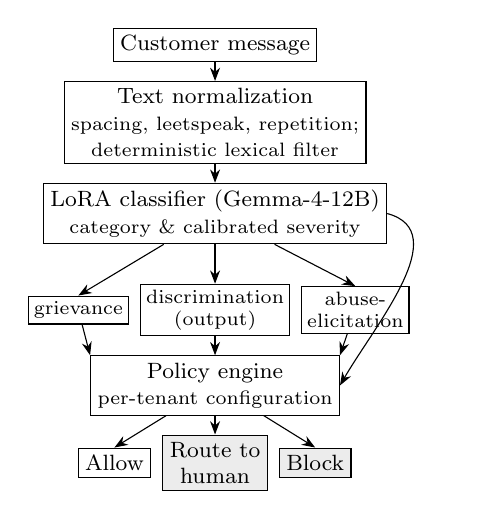
\begin{tikzpicture}[
  node distance=2.4mm and 1.4mm,
  box/.style={draw, rectangle, align=center, font=\footnotesize, inner sep=2.5pt},
  probe/.style={draw, rectangle, align=center, font=\scriptsize, inner sep=2pt},
  act/.style={draw, rectangle, align=center, font=\footnotesize, inner sep=2.5pt},
  >=Stealth
]
\node[box] (msg) {Customer message};
\node[box, below=of msg] (norm) {Text normalization\\{\scriptsize spacing, leetspeak, repetition;}\\{\scriptsize deterministic lexical filter}};
\node[box, below=of norm] (clf) {LoRA classifier (Gemma-4-12B)\\{\scriptsize category \& calibrated severity}};
\node[probe, below=5mm of clf] (disc) {discrimination\\(output)};
\node[probe, left=of disc] (grief) {grievance};
\node[probe, right=of disc] (abuse) {abuse-\\elicitation};
\node[box, below=of disc] (pol) {Policy engine\\{\scriptsize per-tenant configuration}};
\node[act, fill=gray!15, below=of pol] (route) {Route to\\human};
\node[act, left=of route] (allow) {Allow};
\node[act, fill=gray!15, right=of route] (block) {Block};
\draw[->] (msg) -- (norm);
\draw[->] (norm) -- (clf);
\draw[->] (clf) -- (grief.north);
\draw[->] (clf) -- (disc);
\draw[->] (clf) -- (abuse.north);
\draw[->] (grief) -- (pol.north west);
\draw[->] (disc) -- (pol);
\draw[->] (abuse) -- (pol.north east);
\draw[->] (clf.east) to[out=-15,in=60] (pol.east);
\draw[->] (pol) -- (allow.north);
\draw[->] (pol) -- (route);
\draw[->] (pol) -- (block.north);
\end{tikzpicture}
\caption{BankShield pipeline. A customer message is normalized, scored by a LoRA-adapted classifier, three lightweight probes, and a deterministic lexical filter, and mapped by a per-tenant policy engine to one of three actions: allow, route to a human, or block.}
\label{fig:pipeline}
\end{figure}


\section{The \guardaudit{} Protocol}
\label{app:protocol}

\guardaudit{} evaluates a deployed guard in four steps, each with a reporting obligation.

\paragraph{1. Decontaminate.} Remove from every evaluation set any item that exactly matches a training example (on normalized text) and any whose word-level Jaccard similarity to its nearest training neighbor is $\geq 0.70$; report per-set removal counts, and score all systems on the same decontaminated sets (\S\ref{sec:decon}, Appendix~\ref{app:decon}).

\paragraph{2. Pair every detection figure.} Report recall on unsafe items together with the over-block rate on matched benign items, never a detection figure alone, with Wilson 95\% CIs; use McNemar's exact test for paired per-item comparisons and Fisher's exact test for unpaired aggregates (\S\ref{sec:paired}).

\paragraph{3. Audit the guard's own fairness.} Construct counterfactual minimal pairs in which only a protected attribute varies, and report three metrics jointly: flip rate (invariance), over-flag on benign identity mentions, and catch on biased content, so that invariance cannot be satisfied by blindness (\S\ref{sec:fairness}).

\paragraph{4. Evaluate the deployed configuration.} Score the action space the system actually deploys (here allow / route / block), counting designed escalations separately from refusals, and report policy sensitivity where thresholds are tunable (\S\ref{sec:threeway}, \S\ref{sec:policyflex}).

The protocol is model-, language-, and domain-agnostic: steps 1--2 require access to the guard's training data, step 3 a bias benchmark for the deployment locale, and step 4 only the system's action space.

\section{Output-Safety Per-Category Detail}
\label{app:outsafety}
Table~\ref{tab:outputsafety} is, deliberately, the mirror image of Table~\ref{tab:banking}, and we report it as-is. On generic output-safety, BankShield ranks \emph{fourth} of six on paired accuracy (28.8\%): it catches nearly every harmful reply (95.5\%) but over-blocks the benign controls (68.2\%), while purpose-built safety LLMs, Llama Guard 4 (48.5\%) and NemoGuard (47.0\%), are better calibrated because these mainstream harms are squarely in their training distribution. BankShield's blanket strictness, a tunable policy choice (\S\ref{sec:tenant}; under an advisory configuration these over-blocks become non-blocking audit flags), is a genuine calibration cost here, and we do not present it otherwise. One category resists the whole field: on mishandling a distressed customer, NemoGuard, AWS, and PromptGuard score \emph{zero}, and Llama Guard 4 only 2/11, a guard that catches a banking assistant mishandling a customer in distress is nearly absent from current safety tooling, a gap with real stakes in a domain where such conversations occur.



\section{Competence and Ablation Detail}

\begin{table}[t]
\centering
\small
\setlength{\tabcolsep}{3.2pt}
\resizebox{\columnwidth}{!}{%
\begin{tabular}{lcccccc}
\hline
\textbf{Metric} & \textbf{BankSh.} & \textbf{\twelveB} & \textbf{Indic} & \textbf{Base} & \textbf{LG-3} & \textbf{WildG.} \\
\hline
Banking-attack rec. $\uparrow$ & 97 & 98 & 88 & 94 & 94 & 54 \\
XSTest-unsafe rec. $\uparrow$ & 98 & 96 & 89 & 95 & 83 & 90 \\
XSTest-safe o-block $\downarrow$ & 18 & 21 & 46 & 27 & 3 & 2 \\
Banking o-block $\downarrow$ & 0 & 1 & 19 & 4 & 3 & 1 \\
\hline
\end{tabular}}
\caption{Detection and over-block across six systems (four guards, the un-adapted \texttt{gemma-4-12B-it} backbone \twelveB{}, and the un-adapted \texttt{gemma-3-4b-it} Base), neutral data, in \%. Higher recall and lower over-block are better. The un-adapted 12B backbone tracks BankShield closely on banking-attack recall (98 vs 97), XSTest-unsafe recall (96 vs 98), and XSTest-safe over-block (21 vs 18), locating that competence largely in the backbone (\S\ref{sec:fairness}). All systems except WildGuard catch 88--98\% of Indic banking attacks. Banking o-block for BankShield counts block only (with routing counted as refusal it is 16\%); the Indic guard's banking figure macro-averages its English (12\%, n=200) and Hindi/Hinglish (26\%, n=74) subsets. Competitor rows are the authors' runs; per-item logs were not retained. The released package is analysis-only (it regenerates tables from the released logs and includes the rival adapter code for reference); it is not a turnkey execution harness. Wilson 95\% CIs in Table~\ref{tab:ci}.}
\label{tab:main}
\end{table}
\label{app:competence}
\label{sec:competence}

The fairness result of \S\ref{sec:fairness} is meaningful only if BankShield is a competent guard, that is, if it detects the banking attacks it is deployed to stop. We establish that here, against the strongest available guards on neutral data.

\paragraph{Banking-attack recall.} On a neutral set of Indic banking attacks (n=89; English, Hindi, romanized Hindi), BankShield detects 97\%, matching Llama Guard 3 (94\%) and the un-adapted backbone (98\%); even the small \texttt{gemma-3-4b-it} base (94\%) and L3Cube (88\%) are competent, while only WildGuard collapses on Indic input (54\%, $p{=}8{\times}10^{-12}$). Indic banking-attack competence is thus largely a property of a capable backbone, not specialized training: all systems except WildGuard catch 88--98\%. What distinguishes guards is not this competence but fairness (\S\ref{sec:fairness}).

On XSTest's unsafe set (external), BankShield reaches 98\%, highest among the guards but close to the un-adapted backbone's 96\% (Table~\ref{tab:main}), again largely the backbone's.

On over-blocking, we do not lead. On XSTest-safe, Llama Guard 3 (3\%) and WildGuard (2\%) over-block far less than BankShield (18\%). BankShield's 18\% closely tracks the un-adapted \texttt{gemma-4-12B-it} backbone (21\%), so this calibration (and the low benign-banking over-block, 1\% un-adapted, $\approx$0\% for BankShield) is the backbone's, not our adaptation's.

The Indic guard's reported 0.00\% over-refusal rate does not reproduce: with its released model and code we observe 46\% over-blocking on XSTest-safe (Appendix~\ref{app:repro}). We draw only the methodological point: a near-zero over-refusal figure is uninformative unless reported with unsafe-set recall on the same data.

The over-block rates above count only benign content that is blocked (a hard refusal that denies a customer legitimate service), not content routed to a human (a designed escalation for grievance or distress that preserves continuity of service); counting routing as refusal would raise the banking figure to 16\%, but such routing is the intended behaviour, not an error.

\begin{table}[t]
\centering\small\setlength{\tabcolsep}{3.5pt}
\resizebox{\columnwidth}{!}{%
\begin{tabular}{lccccccc}
\hline
\textbf{Recall $\uparrow$} & \textbf{PolyG} & \textbf{HarmB} & \textbf{HH} & \textbf{XST} & \textbf{JbB} & \textbf{ToxC} & \textbf{Pooled} \\
\hline
\textbf{BankShield} & 95 & 100 & 75 & 98 & 100 & 90 & \textbf{90.9} {\footnotesize[89--92]} \\
PolyGuard           & 62 & 92  & 75 & 88 & 96  & 81 & 74.1 {\footnotesize[73--75]} \\
WildGuard           & 36 & 99  & 78 & 91 & 98  & 74 & 73.5 {\footnotesize[73--74]} \\
AWS Bedrock         & 35 & 81  & 57 & 86 & 88  & 92 & 69.0 {\footnotesize[66--72]} \\
L3Cube-IndicGuard   & 61 & 94  & 69 & 89 & 92  & 49 & 67.6 {\footnotesize[67--68]} \\
Qwen3Guard          & 46 & 97  & 61 & 80 & 96  & 56 & 60.2 {\footnotesize[59--61]} \\
Llama Guard 3       & 43 & 97  & 45 & 79 & 94  & 32 & 45.2 {\footnotesize[44--46]} \\
\hline
\end{tabular}}\\[2pt]
\resizebox{\columnwidth}{!}{%
\begin{tabular}{lccccccc}
\hline
\textbf{Over-block $\downarrow$} & \textbf{PolyG} & \textbf{HH} & \textbf{XST} & \textbf{JbB} & \textbf{ToxC} & \textbf{ORB} & \textbf{Pooled} \\
\hline
\textbf{BankShield} & 46 & 2 & 18 & 65 & 14 & 16 & 20.7 {\footnotesize[19--23]} \\
PolyGuard           & 7  & 4 & 5  & 64 & 11 & 11 & 8.0  {\footnotesize[8--8]} \\
WildGuard           & 1  & 1 & 2  & 50 & 6  & 13 & 4.5  {\footnotesize[4--5]} \\
AWS Bedrock         & 24 & 1 & 23 & 38 & 15 & 17 & 16.4 {\footnotesize[14--19]} \\
L3Cube-IndicGuard   & 19 & 7 & 46 & 47 & 5  & 19 & 9.7  {\footnotesize[9--10]} \\
Qwen3Guard          & 1  & 0 & 0  & 14 & 1  & 4  & 1.1  {\footnotesize[1--1]} \\
Llama Guard 3       & 3  & 0 & 3  & 19 & 3  & 1  & 1.7  {\footnotesize[2--2]} \\
\hline
\end{tabular}}
\caption{External-benchmark competence panel: harm recall (top) and benign over-block (bottom), \%, across seven public safety benchmarks, decontaminated per \S\ref{sec:setup}. \emph{Pooled} is the set-size-weighted rate with Wilson 95\% CI; per-set cells are point estimates (per-set counts released). \textbf{Protocol asymmetry, and its direction.} BankShield and AWS are scored on Jaccard-0.70--deduplicated stratified samples (250/class); the open-weight rivals on the full exact-deduplicated sets. The stricter deduplication is applied \emph{only to our rows} and removes our nearest-to-training (hence easiest) items; we flag this sampling asymmetry as a caveat rather than claim it is strictly conservative, and note only that it does not inflate BankShield's rows. BankShield attains the highest harm recall (90.9\%) at the highest over-block (20.7\%); the low-over-block guards reach calibration by missing 40--55\% of harm. JailbreakBench-safe is adversarial-benign and over-blocked by every system (47--65\%). Llama Guard 4 is omitted: its Llama-4 backbone has unstable inference in current \texttt{transformers} releases, so Llama Guard 3 represents the family. The XSTest column (98/18) matches Table~\ref{tab:main}. Sampled-row per-set $n$ (BankShield/AWS), recall: polyguard 250, harmbench 152, hh-rlhf 250, xstest 189, jailbreakbench 49, toxicchat 250; over-block: polyguard 250, hh-rlhf 250, xstest 207, jailbreakbench 34, toxicchat 250, or-bench 250. Open-weight rivals are scored on the full decontaminated sets; per-set counts (aggregate $k/n$, from which the Wilson CIs recompute) are released in \texttt{rivals\_*.json}.}
\label{tab:extcompetence}
\end{table}

\section{General-Fairness Per-Attribute Detail}
\label{app:fairness}
This is the central question of our evaluation. Prior Indic-safety work treats identity as a category of harm to detect; we instead ask whether the guard is itself biased: whether its verdict changes when only a protected attribute (caste, religion, region, gender) varies, silently over-policing some groups. We audit all six systems on counterfactual minimal pairs extending BharatBBQ \citep{tomar2025bharatbbq}. We report three metrics, all on the same output-side framing (the assistant-facing text) so no system is advantaged by our direction-aware design. \emph{Flip} is the fraction of the 160 minimal-pair sets whose verdict changes when only the protected attribute is swapped (content fixed); \emph{over-flag}, the fraction of 185 benign identity-mention items wrongly flagged (counting a block or discrimination-flag, not routing); \emph{catch}, the fraction of 123 biased items correctly flagged. Because BankShield's discrimination detection is output-side by design (\S\ref{sec:direction}), catch spans operating points. For BankShield, catch is the output-side action catch: of the 82 caught items all are blocked and none routed, so block-only catch equals block-or-route catch (66.7\%); the discrimination probe alone flags 50.4\% (62/123), the remaining catches arising from the other output-side detectors. Per-item actions are released.

\begin{table}[t]
\centering
\small
\setlength{\tabcolsep}{3.2pt}
\resizebox{\columnwidth}{!}{%
\begin{tabular}{lcccccc}
\hline
\textbf{Metric} & \textbf{BankSh.} & \textbf{\twelveB} & \textbf{Indic} & \textbf{Base} & \textbf{LG-3} & \textbf{WildG.} \\
\hline
Flip $\downarrow$ & 0.0 & 2 & 19 & 16 & 0 & 0 \\
Over-flag $\downarrow$ & 4.9 & 2 & 13 & 4 & 1 & 0 \\
Catch biased $\uparrow$ & 66.7 & 24 & 56.9 & 33 & 6 & 24 \\
\hline
\end{tabular}}
\caption{Guard fairness on Indian-context counterfactuals, in \%. Arrows indicate the better direction. \twelveB{} is the un-adapted \texttt{gemma-4-12B-it} backbone: it is already near-invariant (flip 2\%) but catches little biased content (24\%), showing that invariance comes from backbone scale while detection (24\% $\rightarrow$ 66.7\%) is what adaptation adds. BankShield combines zero flip (0.0\%) with the highest biased-content catch (66.7\%, on the separate 123-item biased set); measured on different data, these rule out flag-nothing behaviour but do not establish joint per-example fairness. LG-3 (Llama Guard 3) and WildGuard are invariant only by catching almost nothing. All BankShield metrics here are computed in output mode: flip on 160 minimal-pair sets, over-flag on 185 benign items, catch on 123 biased items. BankShield's flip is significantly below the Indic guard's ($p{<}10^{-9}$) and its catch far exceeds both general guards' ($p{<}10^{-14}$), McNemar. Wilson 95\% CIs in Table~\ref{tab:ci}.}
\label{tab:fairness}
\end{table}

Table~\ref{tab:fairness} reveals a clear divide. On flip, BankShield is invariant (0.0\%), as are both general guards (0\%), while the Indic guard flips on 19\% and the base on 16\% (McNemar vs BankShield $p{=}9{\times}10^{-10}$, $6{\times}10^{-8}$). Flip must be read against the any-flag rate on these benign pairs (lower is better): a set can only flip if a guard flags at least one variant, and flagging benign identity content is itself undesirable. BankShield flags none of the 160 benign sets (as do the general guards), the correct behaviour on benign content, whereas the Indic guard and the base flag many (38 and 25) and then treat the groups differently, flipping on 82--100\% of those. Among guards that leave benign pairs alone, what distinguishes BankShield is that it \emph{also} detects biased content: the general guards detect little (Llama Guard 3 6\%, WildGuard 24\%; both $p{<}10^{-14}$), while BankShield catches 66.7\% on the separate 123-item biased set at a 4.9\% over-flag (block-only, per \S\ref{app:parsing}; 5.4\% counting routing). Its catch does not significantly exceed the Indic guard's 56.9\% ($p{=}0.09$). Taken together, 0\% flip on the benign counterfactuals and 66.7\% catch on the biased set rule out simple flag-nothing behaviour, but, measured on different item sets, do not establish joint per-example fairness.

The general guards' invariance is uninformative: they detect little of the biased content a guard must catch, so a guard that cannot recognize a discriminatory loan denial offers no protection. BankShield stays invariant while retaining the ability to detect biased content. To locate the source, we evaluate the un-adapted \texttt{gemma-4-12B-it} backbone on the same pairs: it flips on 2\%, statistically indistinguishable from BankShield's 0\% ($p{=}0.25$), whereas the smaller \texttt{gemma-3-4b-it} base flips on 16\%. The invariance is thus a property of backbone scale, not our adaptation. What training adds is detection: an ablation traces the biased-content catch from the un-adapted backbone's 24\%, to 43\% with the LoRA-adapted classifier (+19), to 66.7\% with the added discrimination probe (+24; Appendix~\ref{app:training}).

\paragraph{Boundaries of the result.} BankShield over-flags benign identity mentions at 4.9\% (block-only; 5.4\% if routing is counted, still above the general guards' 0--1\%, the price of not being insensitive to identity), catches biased content at 66.7\% (output) and 47\% (input), and retains a mild 5-point asymmetry across bias directions (stereotype-consistent vs stereotype-violating framings). We do not claim joint per-example fairness, since flip and catch are measured on separate item sets; the defensible reading is that BankShield leaves benign identity content unflagged (0\% flip) while detecting biased content the general guards miss.


\section{Sensitivity Sweep Detail}
\label{app:sweep}
Sweeping the discrimination threshold (Low/Med/High) over the 40 coded pairs trades catch against false-flag monotonically and never separates: BankShield output paired 15$\rightarrow$7$\rightarrow$4 of 40, input flat at 19--20 of 40 at every setting; AWS 0$\rightarrow$1$\rightarrow$1. At the least-sensitive setting the eight residual control false-flags decompose as threat 3, dangerous 1, abuse 2, AML 1, injection 1, with \emph{none} from the discrimination probe, so even a perfect discrimination threshold cannot separate. WildGuard exposes no sensitivity knob. This isolates the confound to the architecture (adverse-tone across detectors), not calibration.



\begin{table}[t]
\centering
\small
\setlength{\tabcolsep}{4pt}
\resizebox{\columnwidth}{!}{%
\begin{tabular}{lcccc}
\hline
 & \textbf{Indic} & \textbf{Bank.} & \textbf{Fair.} & \textbf{Deploy.} \\
\hline
Llama Guard 3 / ShieldGemma & part. & -- & -- & -- \\
CultureGuard & yes & -- & -- & -- \\
L3Cube-IndicGuard & yes & -- & -- & -- \\
\textbf{BankShield} & yes & yes & yes & yes \\
\hline
\end{tabular}}
\caption{Where prior guards sit on the dimensions this paper addresses: Indic coverage, banking focus, a fairness audit \emph{of the guard itself}, and evaluation in deployment (for BankShield, a live pilot; \S\ref{sec:intro}). CultureGuard (NVIDIA, Llama-based) and L3Cube-IndicGuard (Gemma-based) are distinct systems; we evaluate the latter. (``Fair.'' = fairness audit.)}
\label{app:positioning}\label{tab:positioning}
\end{table}

\section{Cross-Language Detection Detail}
\label{app:crosslang}
The subsets (English 120, Tamil 160) were drawn by uniform random sampling with fixed seeds after decontamination; for Davidson, only hate-labeled items are the unsafe class (offensive excluded); the Tamil subset uses the corpus hate label, deduplicated.
\label{sec:crosslang}

A second question is whether BankShield's detection holds across Indic languages. We test on held-out hate-speech benchmarks in English \citep{davidson2017} and Tamil \citep{tamilhate2024}, decontaminated against our training corpus. These probe cross-script rather than code-mixed competence; our romanized and code-mixed evaluation is concentrated in the banking-attack set (\S\ref{sec:setup}), and extending code-mixed hate-speech evaluation to the Dravidian languages is future work. (We excluded Hindi: the standard benchmark overlapped our training data, which we report in Limitations rather than present as a memorized result.) The pattern is stark. On English hate (Davidson, n=120) the general guards are not weak: WildGuard is in fact the strongest of the three at 98\% [93--99] versus BankShield's 82\% [75--88] and Llama Guard 3's 65\% [56--73]. But on Tamil (n=160) their detection drops sharply: BankShield reaches 84\% [78--89] against Llama Guard 3's 18\% [13--25] and WildGuard's 2\% [1--6] ($p{<}10^{-30}$). The general guards are English-specialized; BankShield stays competent across scripts.

We add a second Dravidian language, Telugu, on a held-out public hate benchmark \citep{teluguhate2022} decontaminated against our corpus: BankShield catches 72\% (55/76) of native-script Telugu hate, a second point of Dravidian competence, at a higher benign over-block (29\% of 150) consistent with the looser non-English calibration of \S\ref{sec:fairness}. For Kannada the picture is different: the public offensive benchmark overlapped our training data as heavily as the Hindi one (all native-script unsafe items matched), so we exclude it. A synthetic benign-only check finds a low over-block (5\%, 4/79) on native Kannada, but a held-out Kannada \emph{unsafe} evaluation, which neither the contaminated public data nor a safety-aligned generator can supply and which machine translation would violate our in-language principle (\S\ref{sec:data}) to obtain, remains future work.

Cross-language competence does not itself confer fairness (the multilingual Indic guard remains identity-sensitive, 19\% flip), so the two results are complementary: \S\ref{sec:fairness} shows fairness on identity swaps; this section shows detection does not depend on English.

Together the results support H1--H3: BankShield is competitive on banking detection, and combines low counterfactual flip with biased-content detection (reported as separate axes, not a joint guarantee), while extending detection to other scripts, though unevenly (Tamil 84\%, Telugu 72\%, but Devanagari Hindi 42.6\% on biased content).




\section{Decontamination Details}
\label{app:decon}

All evaluation sets are decontaminated against 401{,}274 unique training and evaluation texts (525{,}094 rows across 14 files; a superset of the $\approx$172K SFT set of \S\ref{sec:data}, also including the fairness training set and held-out evaluation material) by exact-match on normalized text plus word-level (whitespace-tokenized) Jaccard similarity $\geq$ 0.70; the deduplication script is released with the benchmark artifacts. Removal counts: author-constructed Hindi/Hinglish banking, 6 of 80 removed (74 retained); native-script benign, 0 of 40; Banking-77, 0 (exact and near); XSTest, 0; the fairness benchmark (BharatBBQ), 0 exact and 0 near-duplicate, including against both the 11,907-item fairness training set and the 4,499-item demographic recalibration set that together train the output-side discrimination probe (13,622 safe/discrimination items after label filtering), confirming the fairness result behind the 66.7\% catch is held-out; native hate-speech, 0 overlap for English and Tamil, but 117 of 120 (98\%) for the standard Hindi benchmark, which was consequently excluded (see Limitations). An independent rerun of the near-duplicate step over the released one-way-hashed training index reproduces these figures \emph{approximately}, not exactly: it yields 1{,}978 total Jaccard-$\geq$0.70 near-duplicates against the public benchmarks versus the 1{,}961 in the reported per-set counts (a $\approx$1\% difference attributable to index-rebuild ordering).

\section{Dataset Statistics}
\label{app:stats}

Evaluation sizes (full detail Appendix~\ref{app:decon}): XSTest 250/200; Banking-77 200 benign; Hindi/Hinglish benign 74; native-script benign 40; BharatBBQ 1,056 (185 benign, 123 biased, 160 minimal-pair sets over religion/caste/region/gender); 89 Indic banking attacks.  Banking-77 has no India-specific training lineage; the author-constructed banking and attack sets were verified disjoint from training by the procedure of Appendix~\ref{app:decon}.


All author-constructed sets were written by a single bilingual author with banking-domain familiarity; two independent bilingual annotators re-labeled a 159-item stratified sample blind to the answer key, following a written protocol released with the artifacts (inter-annotator $\kappa=0.97$; see Limitations for the residual authorship-circularity caveat).

\paragraph{Control validation.} We validate the banking control labels in two blind studies. First, on a 120-item stratified sample, an initial reviewer applied a strict construct---treating any adverse decision that names a protected attribute as discriminatory regardless of the stated reason---accepting only 3 of 57 controls (Cohen's $\kappa=0.03$), while a reviewer under clarified instructions (an objective documented reason makes an incidental protected-attribute mention legitimate) agreed with our labels ($\kappa=0.93$); the disagreement is construct-driven. Second, to cover the exact tier behind the 75.0\% control false-flag rate, two independent domain experts blind-labeled all 40 coded pairs (80 items: 40 discriminatory, 40 matched controls). Both accepted essentially every legitimate control (40/40 and 39/40), so the controls are expert-validated and the 75.0\% is a genuine over-flag rate; they agreed with our labels at $\kappa=0.80$ and $0.75$ (expert--expert $\kappa=0.90$), confirming 32/40 and 31/40 of the coded-discriminatory items (the coded-proxy tier is subtle, so some read as borderline---a construct-sensitivity we retain). Reviewers are volunteer bilingual professionals with banking or fairness-evaluation experience who worked independently and blind to the answer key from the written instructions released with the artifacts, with informed consent and no compensation; per-item ratings are released with identities anonymized.

\paragraph{Licenses.} External datasets are used under their published licenses: XSTest, Banking-77, and the Telugu hate-speech corpus under CC-BY-4.0; the Davidson English hate-speech corpus under MIT; the Tamil hate-speech corpus under Apache-2.0; BharatBBQ under the MIT license declared on its official HuggingFace release (which covers the English and Hindi splits we use). Our author-constructed benchmarks contain no items copied from these sources (Appendix~\ref{app:decon}); the released BharatBBQ-derived minimal-pair sets redistribute source items under that license with attribution.

Table~\ref{tab:ci} reports Wilson 95\% confidence intervals for the point estimates in Tables~\ref{tab:main} and~\ref{tab:fairness}.

\begin{table}[t]
\centering
\small
\setlength{\tabcolsep}{4pt}
\resizebox{\columnwidth}{!}{%
\begin{tabular}{lccc}
\hline
\textbf{Metric (system)} & \textbf{n} & \textbf{\%} & \textbf{[95\% CI]} \\
\hline
Banking-attack rec. (BankSh.) & 89 & 97 & [91--99] \\
Banking-attack rec. (\twelveB) & 89 & 98 & [92--99] \\
Banking-attack rec. (Indic) & 89 & 88 & [79--93] \\
Banking-attack rec. (Base) & 89 & 94 & [88--98] \\
Banking-attack rec. (LG-3) & 89 & 94 & [88--98] \\
Banking-attack rec. (WildG.) & 89 & 54 & [44--64] \\
XSTest-unsafe rec. (BankSh.) & 200 & 98.5 & [96--99] \\
XSTest-unsafe rec. (\twelveB) & 200 & 96 & [92--98] \\
XSTest-safe o-block (BankSh.) & 250 & 18 & [14--23] \\
XSTest-safe o-block (Indic) & 250 & 46 & [40--52] \\
XSTest-safe o-block (\twelveB) & 250 & 21 & [16--26] \\
Flip (BankSh.) & 160 & 0.0 & [0--2.3] \\
Flip (\twelveB) & 160 & 2 & [1--6] \\
Flip (Indic) & 160 & 19 & [14--26] \\
Flip (Base) & 160 & 16 & [11--22] \\
Over-flag (BankSh.) & 185 & 4.9 & [3--9] \\
Over-flag (\twelveB) & 185 & 2 & [1--5] \\
Over-flag (Indic) & 185 & 13 & [9--19] \\
Catch biased (BankSh.) & 123 & 66.7 & [58--74] \\
Catch biased (\twelveB) & 123 & 24 & [18--33] \\
Catch biased (Indic) & 123 & 56.9 & [48--66] \\
Catch biased (LG-3) & 123 & 6 & [3--12] \\
Catch biased (WildG.) & 123 & 24 & [17--32] \\
\hline
\end{tabular}}
\caption{Wilson 95\% confidence intervals for the main point estimates in Tables~\ref{tab:main}--\ref{tab:fairness}. Percentages are exact where non-integer. Cross-language hate-speech CIs are given inline in Appendix~\ref{app:crosslang}.}
\label{tab:ci}
\end{table}

\paragraph{Confidence intervals for the banking and output-safety tables.}
\label{app:ci-extra}
Wilson 95\% intervals for BankShield's headline rates in Tables~\ref{tab:banking} and~\ref{tab:outputsafety}. Banking (\S\ref{sec:banking}): explicit catch 100\% [89.3, 100], coded catch 97.2\% [86, 100], control false-flag 75.0\% [59, 86], paired 20.0\% [10, 35]. Output-safety (\S\ref{sec:outputsafety}): catch 95.5\% [87.5, 98.4], over-block 68.2\% [56.2, 78.2], paired 28.8\% [19.3, 40.6]. On these $n{=}36$--$66$ sets the intervals are wide; we read the banking and output-safety point estimates as directional accordingly.

\section{Baseline Systems}
\label{app:baselines}

All baselines are evaluated on the same decontaminated sets as BankShield and appear directly in Tables~\ref{tab:main}--\ref{tab:fairness}: L3Cube-IndicGuard (run with its released inference script), the un-adapted \texttt{gemma-3-4b-it} base model, Llama Guard 3 (8B), and WildGuard (7B). Prompt-Guard (86M) was evaluated but excluded from the tables as scope-mismatched: it is a jailbreak/injection detector and is inert on this content-safety evaluation (flagging none of the benign or the toxicity/violence content under its intended configuration), so reporting it alongside content-safety guards would mislead.

\section{Reproduction of a Reported Over-refusal Figure}
\label{app:repro}

The Indic guard's accompanying work \citep{bramhecha2026} reports a 0.00\% over-refusal rate on XSTest safe prompts. Running its released model with its released inference script and prompt format on the XSTest-safe set, we observe a 46\% over-block rate (95\% CI [40--52]). Illustrative benign prompts it flags include innocuous questions rephrased with sensitive surface words. We do not adjudicate the discrepancy with the reported figure, which may reflect a different definition of over-refusal; we report only what the released artifacts produce, and use it solely to motivate reporting over-block together with unsafe-set recall on the same data.

\section{Output Parsing and Decision Mapping}
\label{app:parsing}

BankShield uses greedy decoding (\texttt{do\_sample=False}); its category and severity are obtained from a single forward pass by scoring log-probabilities over a fixed set of label tokens rather than by free-form generation, and its probes are sigmoid scores over sentence embeddings. All decoding is deterministic, so results are seed-independent and no sampling seed is involved. Comparison systems are run greedily with a 96-token generation budget and parsed from JSON by regular expression; on L3Cube-IndicGuard this yielded 0 parse errors over 764 items. For the decision mapping, a comparison system's unsafe label is treated as a flag; for BankShield, a block or route is treated as a flag, with over-block rates counting block only and routing reported separately.
The un-adapted backbones (12B$_0$ and the 4B base) are scored with the same deterministic
label-token procedure and instruction template as BankShield's classifier, differing only
in the absence of the LoRA adapter and probes.

\section{Training and Deployment Details}
\label{app:training}

\paragraph{Classifier adaptation.} BankShield adapts \texttt{google/gemma-4-12B-it} with LoRA (rank $r{=}16$, $\alpha{=}32$, dropout 0.05; target modules: the attention projections q, k, v, o and the MLP gate, up, down), served in 4-bit NF4 with double-quantization and bfloat16 compute.
Training used AdamW with a learning rate of $2{\times}10^{-4}$ on a cosine schedule (warmup ratio 0.03), one epoch over the $\approx$172K-example corpus, an effective batch size of 32 (8$\times$4 gradient accumulation), and a maximum sequence length of 128 tokens, on a single NVIDIA A4000 (16\,GB).

\paragraph{Probes.} The three learned probes (grievance, output-side discrimination, abuse-elicitation) are logistic-regression heads over 768-dimensional \texttt{intfloat/multilingual-e5-base} embeddings (input formatted as \texttt{query:} + text, truncated to 192 tokens, mean-pooled and L2-normalized), trained with balanced class weights; a fourth signal is a deterministic normalized-lexicon match. Per-probe thresholds are stored in configuration and tunable per tenant.
The output-side discrimination probe is trained on 13{,}622 safe/discrimination-labelled items (4{,}546 discrimination, 9{,}076 safe) drawn from two in-house synthetic sources: the fairness training set (\S\ref{sec:data}) and a counterfactual-balanced demographic recalibration set. Both sources are verified disjoint from the BharatBBQ evaluation data (0 exact and 0 word-level Jaccard $\geq$ 0.70 near-duplicates across all 1{,}102 evaluation items; Appendix~\ref{app:decon}), so the 66.7\% catch is a held-out result.
An ablation decomposes the biased-content catch (n$=$123, output mode) across components: the un-adapted \texttt{gemma-4-12B-it} backbone catches 24\%; LoRA fine-tuning raises the classifier alone to 43\% (+19); adding the output-side discrimination probe raises the full system to 66.7\% (+24), recovering 29 cases the classifier misses. Counterfactual invariance, over-block, and attack recall are, by contrast, inherited from the backbone (\S\ref{sec:fairness}), so fine-tuning's distinctive contribution is biased-content detection: the probe is its decisive component, though not its sole source.

\paragraph{Deployment status.} BankShield runs as a self-hosted live pilot on a single on-premise NVIDIA A4000 (16 GB), serving a small number of volunteer testers (former colleagues of an author, not real banking customers); to date it has handled 283 moderation events (snapshot 8 July 2026). The self-hosted, on-premise configuration is what satisfies the localization constraint of \S\ref{sec:reg}. This is an unoptimized pilot, not a production deployment: on this hardware end-to-end latency is p50 $\approx$ 0.7 s / p95 $\approx$ 3.2 s, which production use would reduce with a larger GPU and request batching. The deployment claims in this paper refer to this pilot and its regulatory constraints, not to production scale, and the market figures in \S\ref{sec:intro} describe the setting BankShield targets, not its current user base.

\paragraph{Per-policy action counts (\S\ref{sec:policyflex}).} On the fixed 100-item slice, the same frozen model and probes under three tenant policies (no retraining) yield: strict, 96 blocks; deployed-default, block-first; permissive-advisory, monitor-first (39 route, 37 flag, 12 block, 12 allow). 84 of 100 items change action across policies, and the permissive-advisory policy fully allows 2 items that arguably warrant a flag.

\end{document}
